\documentclass[12pt]{article}
\usepackage[english]{babel}
\usepackage{mathtools}
\usepackage{graphicx}
\usepackage{pdfpages}
\usepackage{subcaption}
\usepackage{float}
\usepackage{natbib}
\usepackage[thinc]{esdiff}
\usepackage{url}
\usepackage[utf8x]{inputenc}
\usepackage{amsmath}
\usepackage{graphicx}
\graphicspath{{images/}}
\usepackage{parskip}
\usepackage{fancyhdr}
\usepackage{vmargin}
\usepackage{listings}
\usepackage{color} %red, green, blue, yellow, cyan, magenta, black, white
\definecolor{mygreen}{RGB}{28,172,0} % color values Red, Green, Blue
\definecolor{mylilas}{RGB}{170,55,241}


\setmarginsrb{3 cm}{2.5 cm}{3 cm}{2.5 cm}{1 cm}{1.5 cm}{1 cm}{1.5 cm}
\usepackage{listings}
\title{Non-linear Control}
\author{Akwasi A. Obeng}                    
\date{December 08, 2019}										
\makeatletter
\let\thetitle\@title
\let\theauthor\@author
\let\thedate\@date

\makeatletter
\renewcommand*\env@matrix[1][\arraystretch]{%
  \edef\arraystretch{#1}%
  \hskip -\arraycolsep
  \let\@ifnextchar\new@ifnextchar
  \array{*\c@MaxMatrixCols c}}
\makeatother


\pagestyle{fancy}
\fancyhf{}
\rhead{\theauthor}
\lhead{\thetitle}
\cfoot{\thepage}

\begin{document}

%%%%%%%%%%%%%%%%%%%%%%%%%%%%%%%%%%%%%%%%%%%%%%%%%%%%%%%%%%%%%%%%%%%%%%%%%%%%%%%%%%%%%%%%%

\lstset{language=Matlab,%
    %basicstyle=\color{red},
    breaklines=true,%
    morekeywords={matlab2tikz},
    keywordstyle=\color{blue},%
    morekeywords=[2]{1}, keywordstyle=[2]{\color{black}},
    identifierstyle=\color{black},%
    stringstyle=\color{mylilas},
    commentstyle=\color{mygreen},%
    showstringspaces=false,%without this there will be a symbol in the places where there is a space
    numbers=left,%
    numberstyle={\tiny \color{black}},% size of the numbers
    numbersep=9pt, % this defines how far the numbers are from the text
    emph=[1]{for,end,break},emphstyle=[1]\color{red}, %some words to emphasise
    %emph=[2]{word1,word2}, emphstyle=[2]{style},    
  }


\begin{titlepage}
	\centering
    \vspace*{0.5 cm}
    
\includegraphics[scale = 0.1]{./uon.jpeg}\\[1.0 cm]	% University Logo
    \textsc{\LARGE ENPM662(Robot Modelling)}\\[2.0 cm]	% University Name
	\textsc{\Large Formal Report}\\[0.5 cm]				% Course Code
	\textsc{\large Project}\\[0.5 cm]				% Course Name
	\rule{\linewidth}{0.2 mm} \\[0.4 cm]
	{ \huge \bfseries \thetitle}\\
	\rule{\linewidth}{0.2 mm} \\[1.5 cm]
	
	\begin{minipage}{0.4\textwidth}
		\begin{flushleft} \large
			\emph{Author:}\\
			\theauthor
			\end{flushleft}
			\end{minipage}~
			\begin{minipage}{0.4\textwidth}
			\begin{flushright} \large
			\emph{UID:} \\
			117000801									% Your Student Number
		\end{flushright}
	\end{minipage}\\[2 cm]
	
	{\large \thedate}\\[2 cm]
 
	\vfill
	
\end{titlepage}

%%%%%%%%%%%%%%%%%%%%%%%%%%%%%%%%%%%%%%%%%%%%%%%%%%%%%%%%%%%%%%%%%%%%%%%%%%%%%%%%%%%%%%%%%

\tableofcontents
\pagebreak

%%%%%%%%%%%%%%%%%%%%%%%%%%%%%%%%%%%%%%%%%%%%%%%%%%%%%%%%%%%%%%%%%%%%%%%%%%%%%%%%%%%%%%%%%

\section{Problem Statement}
%\begin{figure}[H],

    %\centering
    %\textbf{your title}\par\medskip
    %\includegraphics[scale = 0.2]{welding.png}\\[0.0 cm]	% University Logo
    %\caption{Welding in Automotive industry} 
%\end{figure}

\section{Dynamics(Question A)}
\subsection{Lagrangian}  
\textbf{Potential Energy}  \\ \\
The potential energy associated with $m_1$,$M$ and $m_2$ are written obtained as follows.
Setting a reference point of U= 0 at the origin  we get
\begin{align} 
  V_{m_1} &= -m_1*l_1cos(\theta _1(t)) \\
  V_{m_2} &= -m_2*l_2cos(\theta _2(t)) \\
  V_M &=0 \\
  V &= V_{m_1} +V_{m_2} + V_M
\end{align}


\textbf{Kinetic Energy}  \\ \\
The Kinetic energy associated with $m_1$,$M$ and $m_2$ are written obtained as follows
\begin{align}   
  T_{m_1} &= \frac{1}{2}m_1(\diff{x(t)}{t})^2 + \frac{1}{2}m_1l_1^2(\diff{\theta _1}{t})^2 -m_1l_1\cos \theta _1(t) \diff{\theta _1}{t} \diff{x}{t}\\
  T_{m_2} &= \frac{1}{2}m_2(\diff{x(t)}{t})^2 + \frac{1}{2}m_2l_2^2(\diff{\theta _2}{t})^2 -m_2l_2\cos \theta _2(t) \diff{\theta _2}{t} \diff{x}{t}\\
  T_M &= \frac{1}{2}M(\diff{x}{t})^2 \\
  T &= T_{m_1} +T_{m_2} + T_M 
\end{align}


\textbf{Lagrangian}  \\ \\
The lagrangian is calculated as $T - V$ and is obtained as follows

 \begin{align}
   L &= T -V \\
     &= \frac{1}{2}m_1(\diff{x(t)}{t})^2 + \frac{1}{2}m_1l_1^2(\diff{\theta _1}{t})^2 -m_1l_1\cos \theta _1(t) \diff{\theta _1}{t} \diff{x}{t} + \nonumber \\
     &\quad \frac{1}{2}m_2(\diff{x(t)}{t})^2 + \frac{1}{2}m_2l_2^2(\diff{\theta _2}{t})^2 -m_2l_2\cos \theta _2(t) \diff{\theta _2}{t} \diff{x}{t} + \nonumber \\
     &\quad \frac{1}{2}M(\diff{x}{t})^2  +m_1*l_1cos(\theta _1(t)) + m_2*l_2cos(\theta _2(t))
 \end{align}                       


\subsection{Equation of Motion}
\begin{align}
  0&=-m_1l_1\diff[2]{x}{t}\cos \theta _1(t) + m_1l_1^2\diff[2]{\theta _1}{t} + mgl_1\sin \theta _1(t)\\
  0&=-m_2l_2\diff[2]{x}{t}\cos \theta _2(t) + m_2l_2^2\diff[2]{\theta _2}{t} + mgl_22\sin\theta _2(t) \\
  F&= \diff[2]{x(t)}{t}[M+m_1+m_2] -m_1l_1[\diff[2]{\theta _1(t)}{t}cos(\theta _1(t))-\sin \theta _1(t)(\diff{\theta _1}{t})^2]  \nonumber \\
   &-m_2l_2[\diff[2]{\theta _2}{t}\cos \theta _2(t) - \sin \theta_ 2(t) (\diff{\theta _2}{t})^2].
\end{align}
\textbf{NB.Refer to Appendix(Code for Dynamics) on how this was obtained} \\ \\
The equations obtained above can be further simplified to obtain the equation stated below \\ \\
\textbf{Simplification}\\
Make $\diff[2]{\theta_2(t)}{t}$ and $\diff[2]{\theta_1(t)}{t}$ the subject of equations 11 and 12 respectively. Then substitute into equation 13 to get the equation below. \\
\begin{align} 
  \diff[2]{x}{t} &= \frac{-\frac{g}{2}[m_1\sin(2\theta_1(t))+m_2sin(2\theta_2(t))]-m_1l_1\sin(\theta_1(t))(\diff{\theta_1(t)}{t})^2 - m_2l_2\sin(\theta_2(t))(\diff{\theta_2}{t})^2 + F}{M+m_1\sin^2(\theta_1(t)) +m_2\sin^2(\theta_2(t))} 
\end{align} \\
Resubstitue the equation above into equation 11 and 12 to get the following.
\begin{align}
  \diff[2]{\theta_1}{t} &= \frac{\frac{cos(\theta_1)}{l_1}(F-\frac{m_1g\sin(2\theta_1)}{2}-\frac{m_2g\sin(2\theta_2)}{2}-m_1l_1\sin\theta_1(\diff{\theta_1}{t})^2-m_2l_2\sin\theta_2(\diff{\theta_2}{t})^2)}
                           {M+m_1\sin^2(\theta_1(t)) +m_2\sin^2(\theta_2(t))} \\
  \diff[2]{\theta_2}{t} &= \frac{\frac{cos(\theta_2)}{l_2}(F-\frac{m_1g\sin(2\theta_1)}{2}-\frac{m_2g\sin(2\theta_2)}{2}-m_1l_1\sin\theta_1(\diff{\theta_1}{t})^2-m_2l_2\sin\theta_2(\diff{\theta_2}{t})^2)}
                           {M+m_1\sin^2(\theta_1(t)) +m_2\sin^2(\theta_2(t))} 
\end{align}


\newpage
\section{Linearization (Question B)}
A non linear system,$F(X,U)$ with state space euation 
$
  \diff{X}{t} = F(X,U)
$
can be linearized with the equation stated below.

\begin{equation}
  \delta _x = A_F \diff{x(t)}{t} + B_F\diff{x(t)}{t}
\end{equation}
where $A_F =\nabla_xF$,$B_F = \nabla_uF$, U(input) and X(State) \\ \\
Given the equation above, the following state space is chosen for the Dynamic problem.

\begin{align}
  X &=
  \begin{bmatrix}
    x& \diff{x}{t} & \theta_1 & \diff{\theta_1}{t} &\theta_2&\diff{\theta_2}{t}
  \end{bmatrix}^T
\end{align}

Therefore, the state space equation can be written as
\begin{align}
  \diff{X}{t}&= \diff{}{t}
  \begin{bmatrix}[1.5]
    x \\
    \diff{x}{t} \\
    \theta_1 \\
    \diff{\theta_1}{t} \\
    \theta_2\\
    \diff{\theta_2}{t}
  \end{bmatrix} 
  =
  \begin{bmatrix}[1.5]
    f_1(X,U)\\
    f_2(X,U)\\
    f_3(X,U)\\
    f_4(X,U)\\
    f_5(X,U)\\
    f_6(X,U)
  \end{bmatrix} = F
\end{align}
Based on equation above, the following can be noted
\begin{align}
  f_1(X,U) &= \diff{x}{t} \\
  f_2(X,U) &= \diff[2]{x}{t} \quad \text{Refer to Dynamics for equation} \\
  f_3(X,U) &= \diff{\theta}{t} \\
  f_4(X,U) &= \diff[2]{\theta_1}{t} \quad \text{Refer to Dynamics for equation} \\
  f_5(X,U) &= \diff{\theta _2}{t}\\
  f_6(x,U) &= \diff[2]{\theta _2}{t}\quad \text{Refer to Dynamics for equation} \\
\end{align}

From $A_F = \nabla_xF=\frac{\partial F}{\partial X}$ and $B_F=\nabla_uF=\frac{\partial F}{\partial U}$ we get 
\begin{align}
  A_F&=
  \begin{bmatrix}[1.5]
   0 &1 &0 &0 &0 &0 \\
   0 &0 &-\frac{m_1g}{M} &0 &-\frac{m_2g}{M} &0 \\
   0 &0 &0 &1 &0 &0 \\
   0 &0 &-\frac{g}{l_1}(1+\frac{m_1}{M}) &0 &\frac{-m_2g}{l_1M} &0  \\
   0 &0 &0 &0 &0 &1 \\
   0 &0 &\frac{-m_1g}{l_2M} &0 &-\frac{g}{l_1}(1+\frac{m_2}{M}) &0 
  \end{bmatrix}
 \quad
  B_F =
  \begin{bmatrix}[1.5]
    0\\
    \frac{1}{M} \\
    0 \\
    \frac{1}{Ml_1}\\
    0 \\
    \frac{1}{Ml_2}
  \end{bmatrix}
\end{align}
\section{Controllability (Question C)}
\textbf{Output}
\begin{figure}[H]
    \centering
    \textbf{Output of langrange Dynamics}\par\medskip
    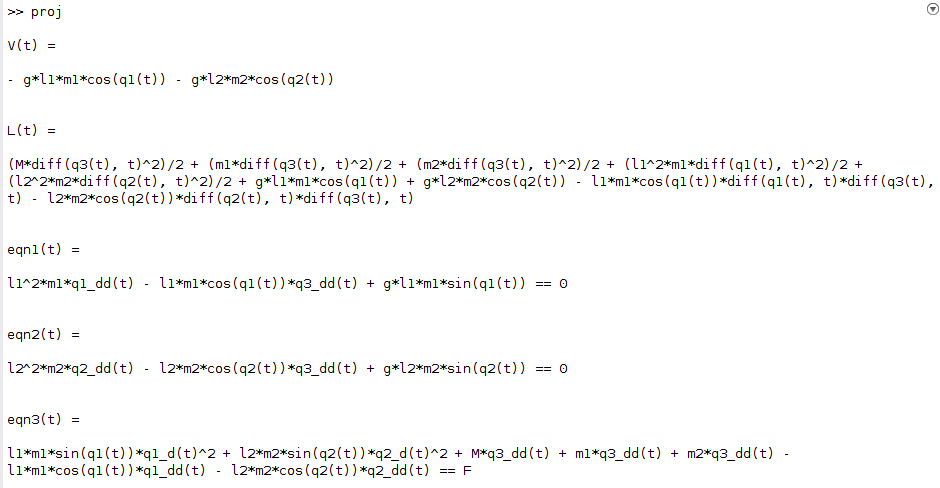
\includegraphics[scale = 0.5]{lagrange.png}\\[0.0 cm]	% University Logo
    \caption{lagrange Dynamics} 
\end{figure}

\section{FeedBack and Linear Quadratic Regulator (Question D)}
\section{Observability (Question E)}


\section{Luenberger Observer (Question F)}
\begin{figure}[H]
    \centering
    \textbf{State x(t) Linear Response}\par\medskip
    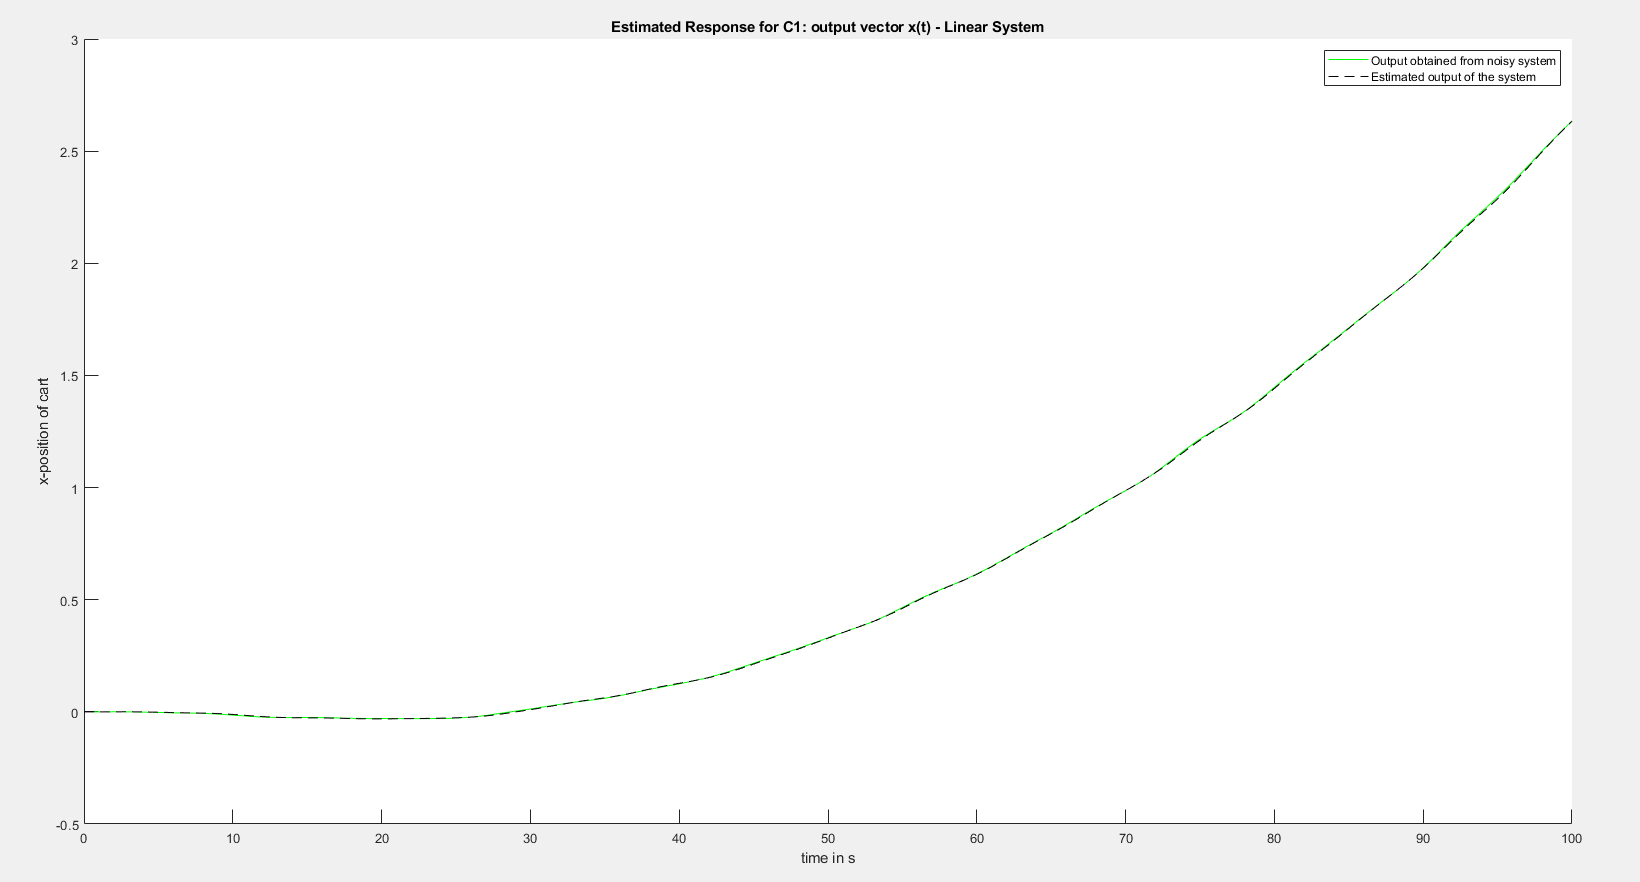
\includegraphics[scale = 0.35]{StateXlinearResponse.png}\\[0.0 cm]	% University Logo
    \caption{State x(t) Linear Response} 
\end{figure}

\begin{figure}[H]
    \centering
    \textbf{State x(t) Non Linear Response}\par\medskip
    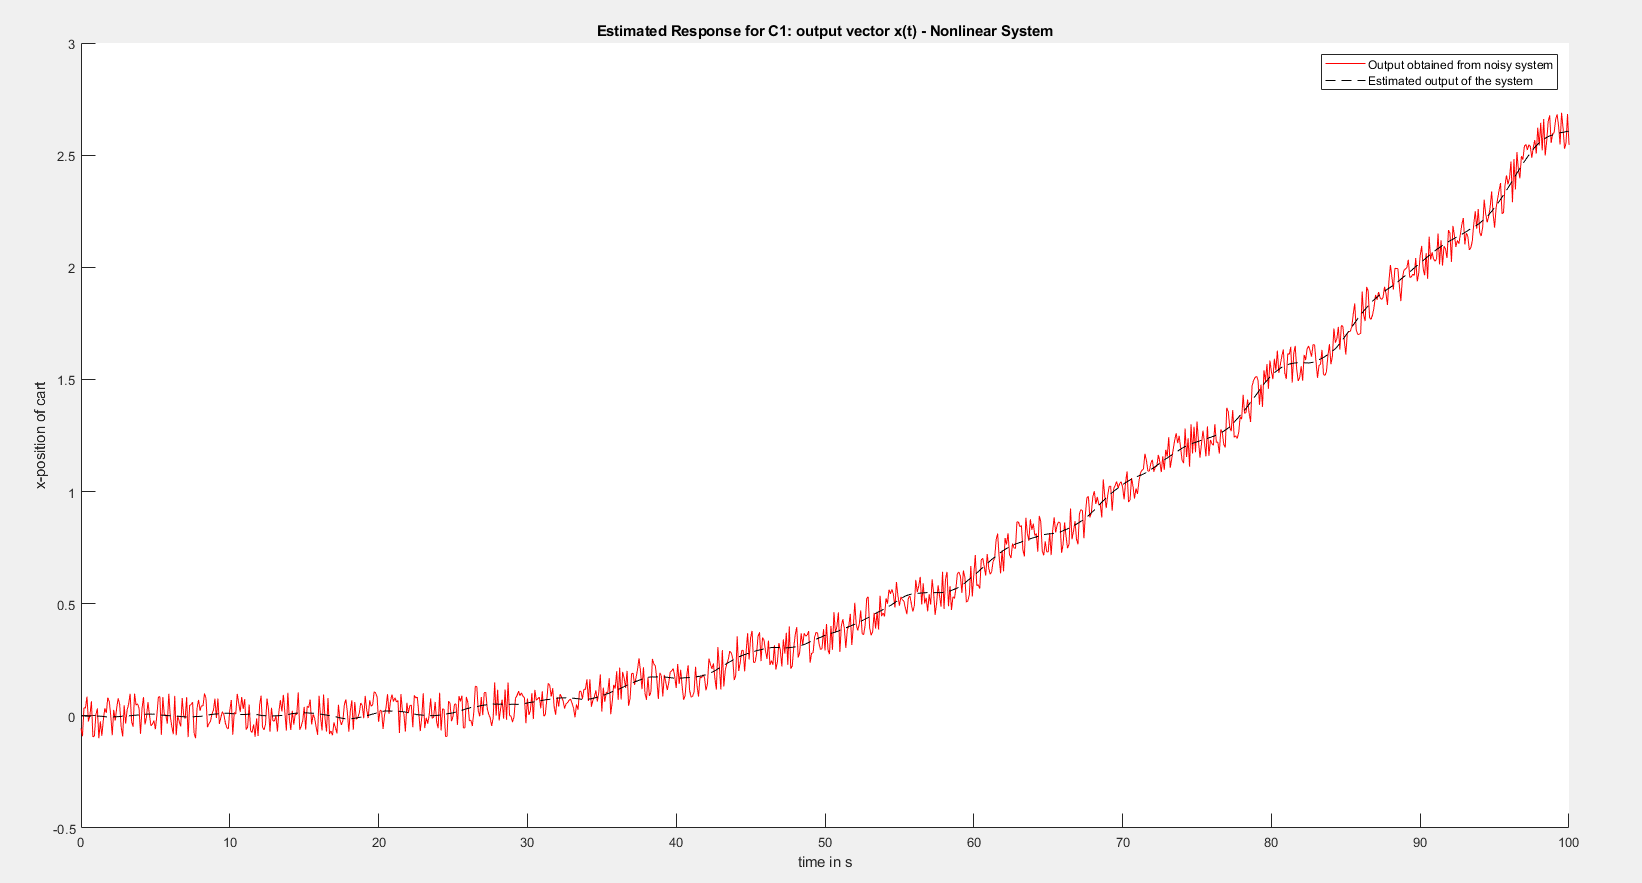
\includegraphics[scale = 0.35]{StateXNonLinearResponse.png}\\[0.0 cm]	% University Logo
    \caption{State x(t) Non Linear Response} 
\end{figure}

\begin{figure}[H]
    \centering
    \textbf{State x(t) and $\theta_2(t)$ Linear Response}\par\medskip
    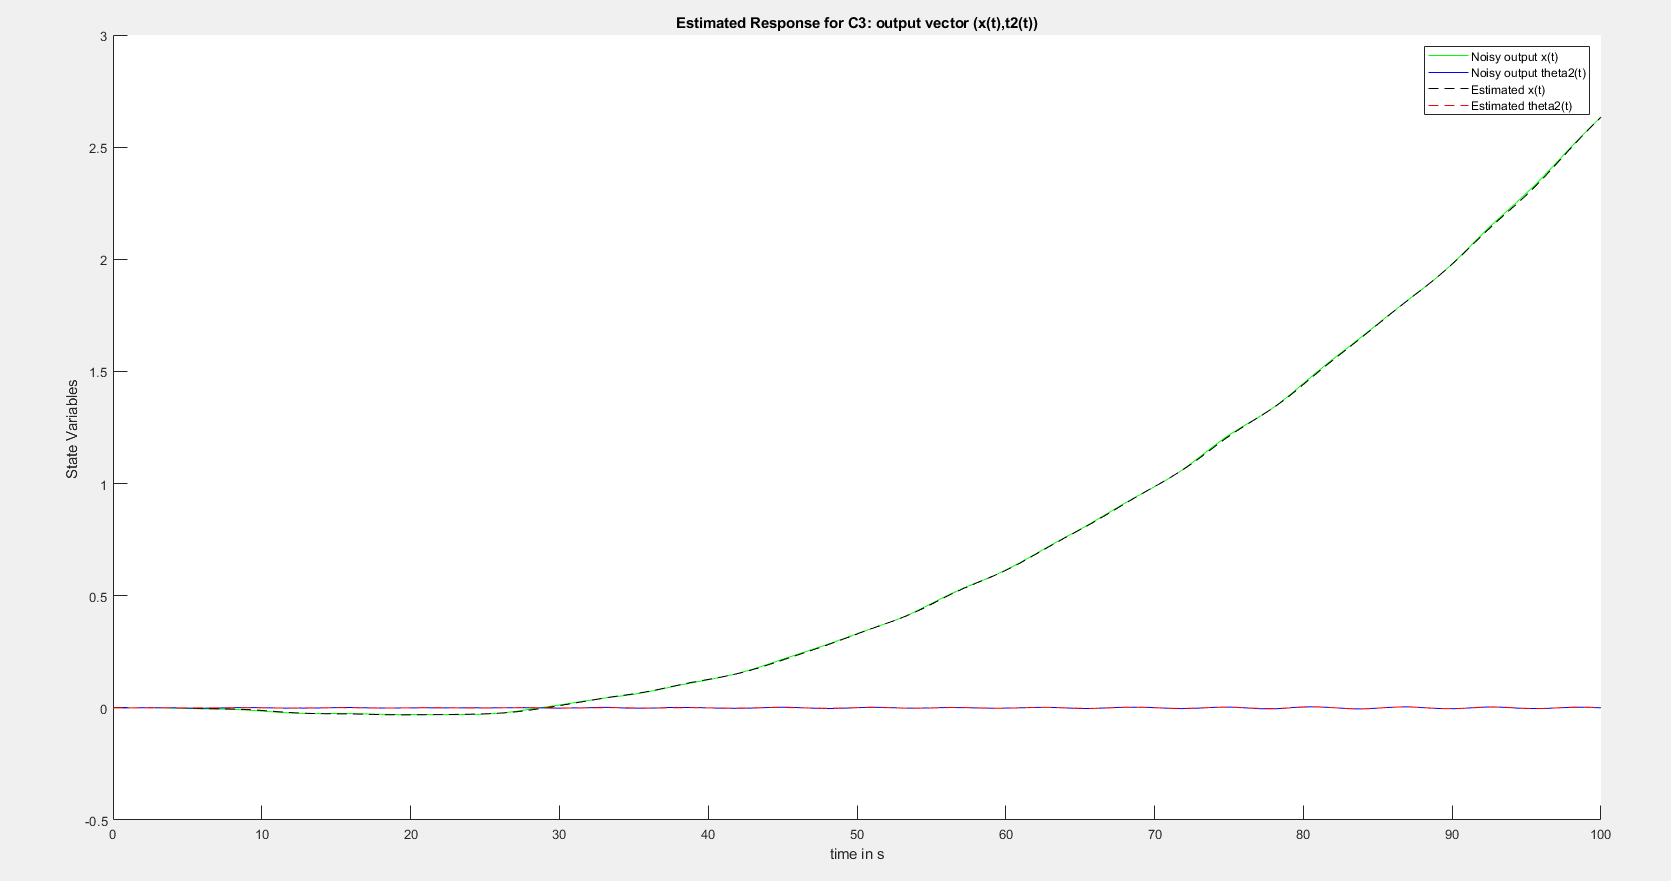
\includegraphics[scale = 0.35]{StateXth2LinearResponse.png}\\[0.0 cm]	% University Logo
    \caption{State x(t) and $\theta_2(t)$ Linear Response} 
\end{figure}

\begin{figure}[H]
    \centering
    \textbf{State x(t) and $\theta_2(t)$ Non-Linear Response}\par\medskip
    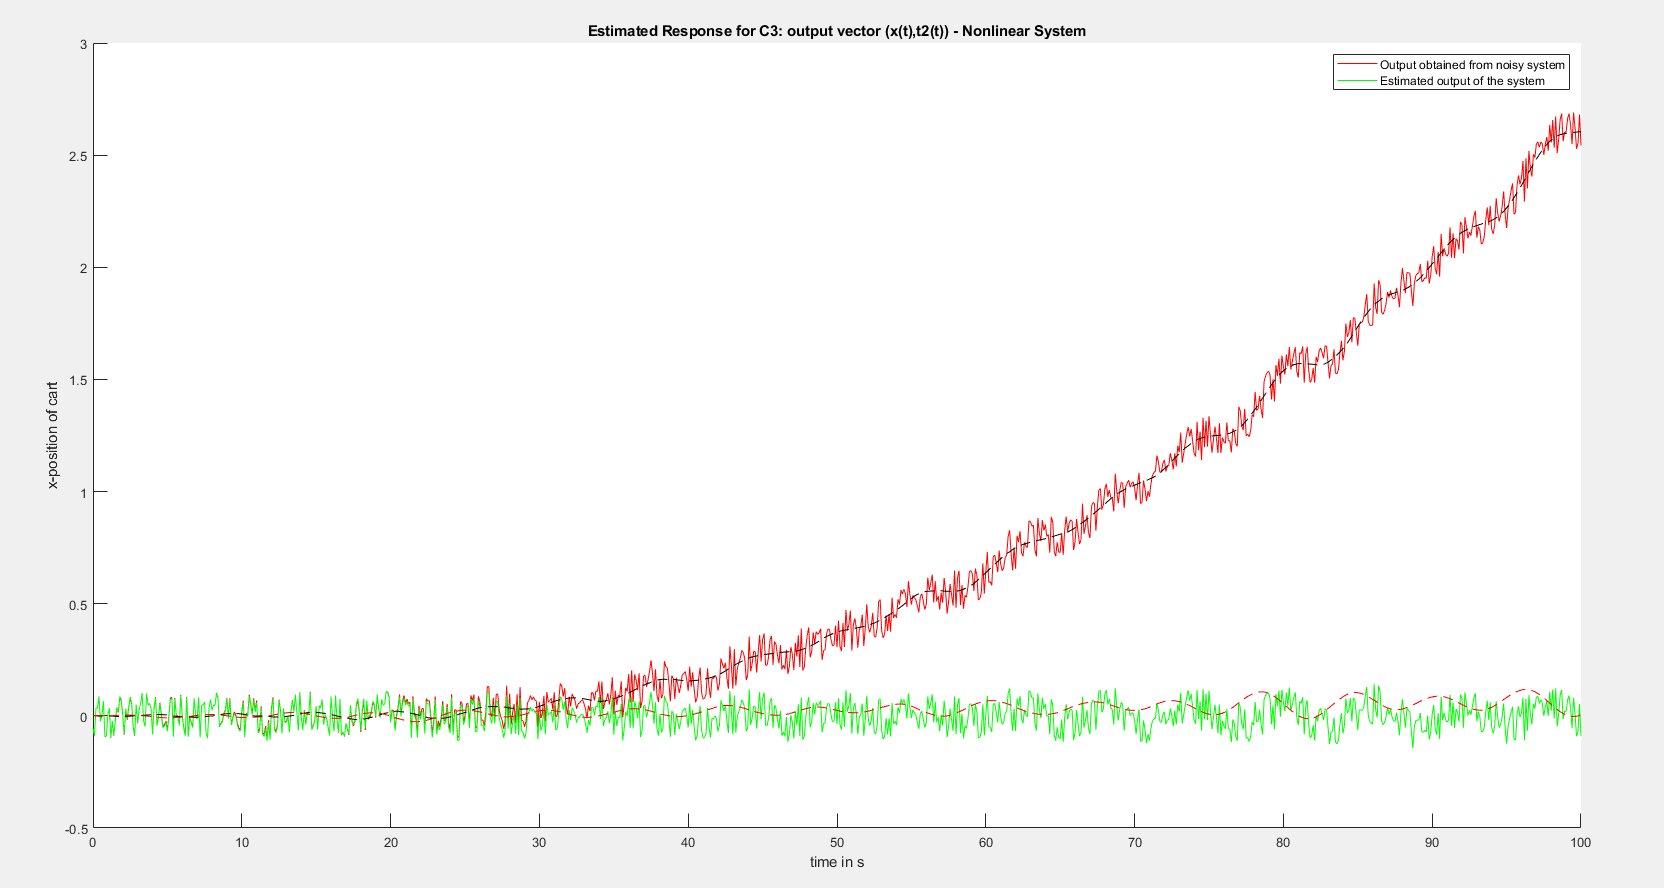
\includegraphics[scale = 0.35]{StateXth2NonLinearResponse.png}\\[0.0 cm]	% University Logo
    \caption{State x(t) and $\theta_2(t)$ Non-Linear Response} 
\end{figure}

\begin{figure}[H]
    \centering
    \textbf{State x(t),$\theta_1(t)$ and $\theta_2(t)$ Linear Response}\par\medskip
    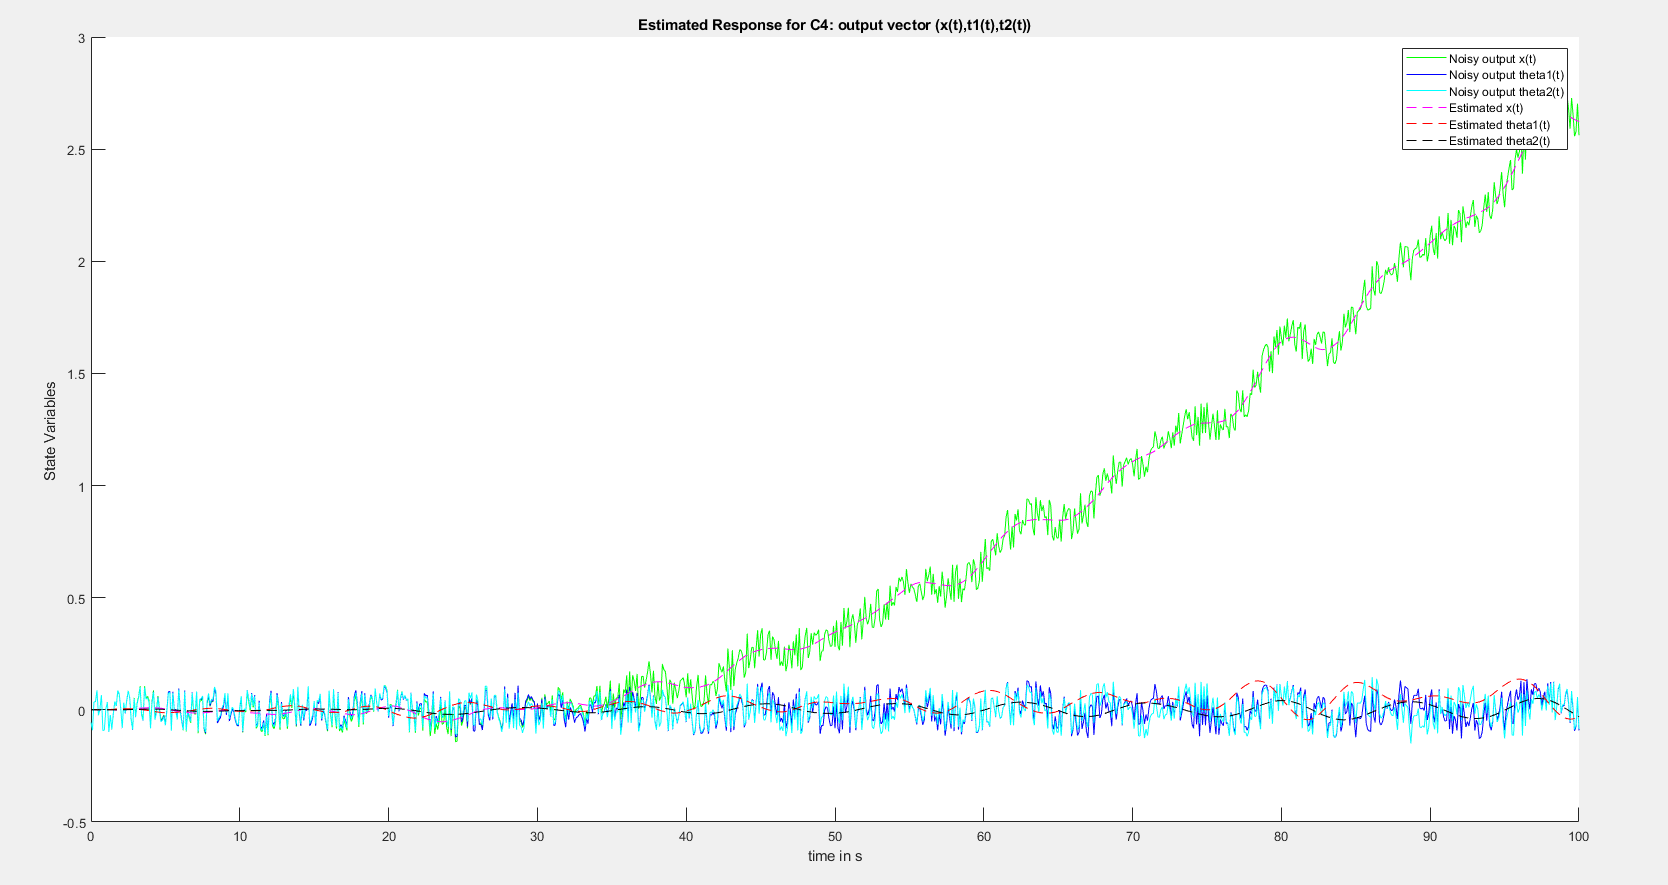
\includegraphics[scale = 0.35]{StateXth1th2NonLinearResponse.png}\\[0.0 cm]	% University Logo
    \caption{State x(t),$\theta_1t()$ and $\theta_2(t)$ Linear Response} 
\end{figure}

\begin{figure}[H]
    \centering
    \textbf{State x(t),$\theta_1(t)$ and $\theta_2(t)$ Non-Linear Response}\par\medskip
    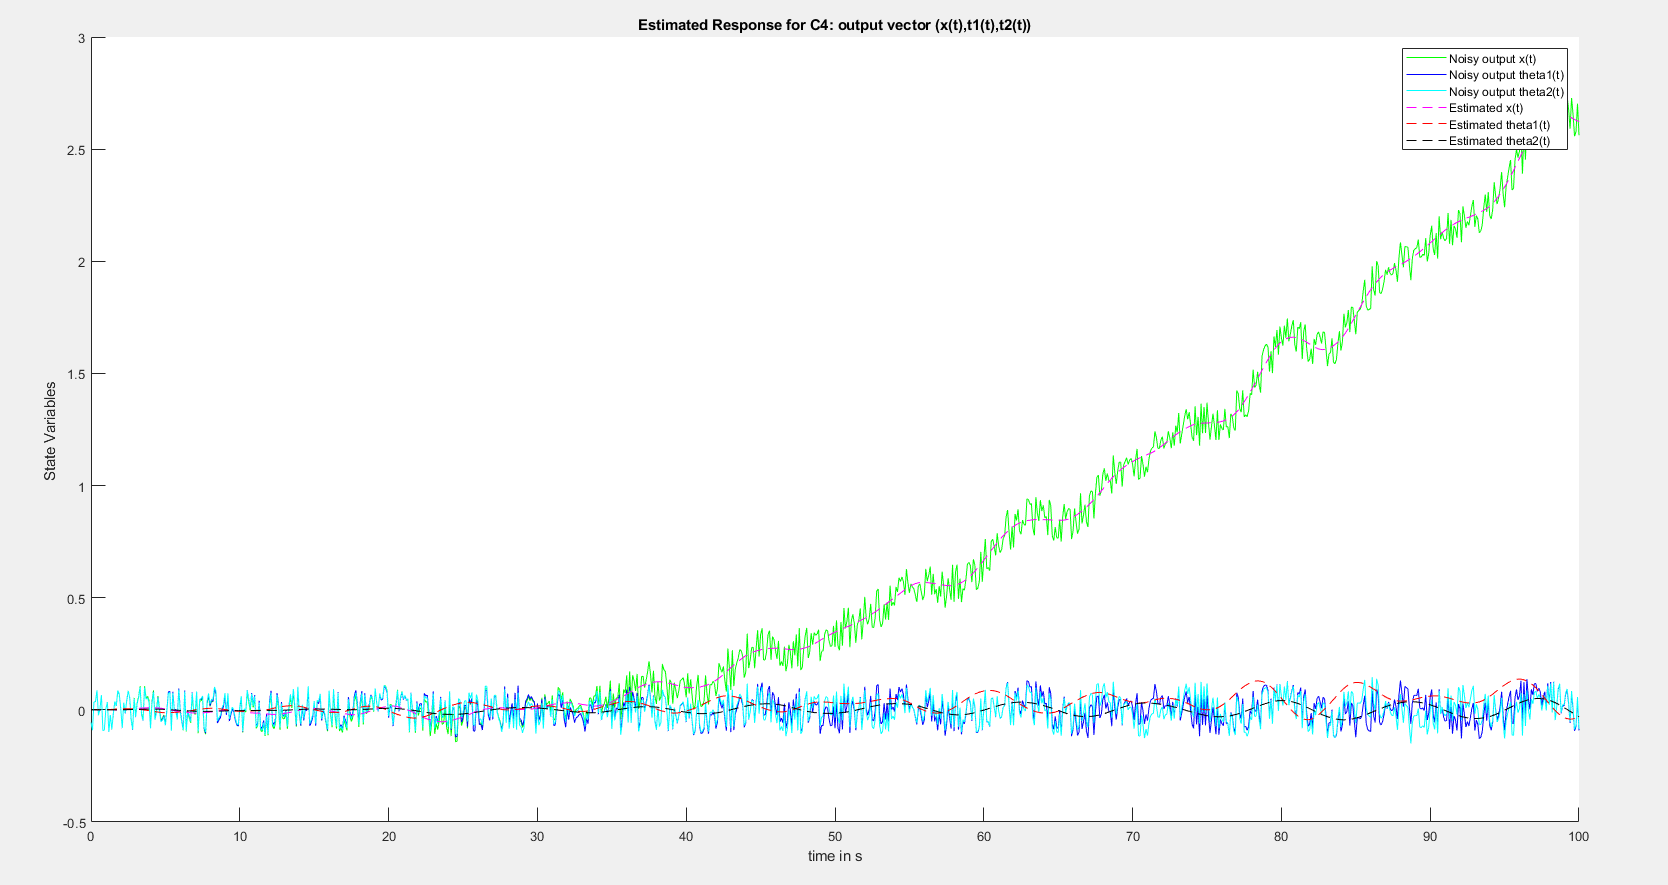
\includegraphics[scale = 0.35]{StateXth1th2NonLinearResponse.png}\\[0.0 cm]	% University Logo
    \caption{State x(t),$\theta_1t()$ and $\theta_2(t)$ Non-Linear Response} 
\end{figure}

\section{LQG (Question G)}

\section{Appendix}
\subsection{Code for Dynamics Calculations}
%\lstinputlisting{proj.m}

\textbf{Output}
\begin{figure}[H]
    \centering
    \textbf{Output of langrange Dynamics}\par\medskip
    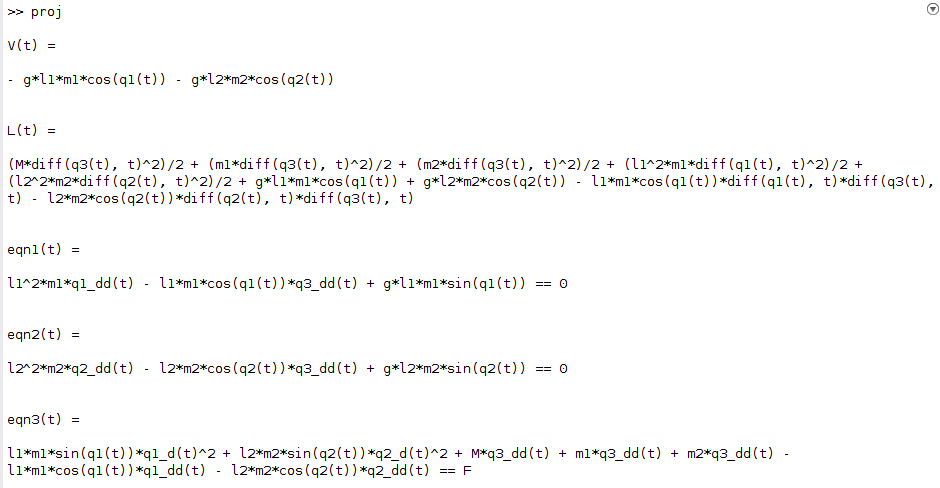
\includegraphics[scale = 0.5]{lagrange.png}\\[0.0 cm]	% University Logo
    \caption{lagrange Dynamics} 
\end{figure}

\subsection{Code for LQR}
%\lstinputlisting{compute.m}

\subsection{Code for LQG}
%\begin{lstlisting}
%\end{lstlisting}

\end{document}
